

%----------------------------------------------------------------------------------------
%  Introduction
%----------------------------------------------------------------------------------------
\chapter{Methodology}
\section{Introduction}
Developing a product configurator is by any means no easy feat. Building it using 3d technology may be even harder. When doing a small documentary analysis to get and set a proper theoretical framework, it became abundantly clear that there is a lot of research done into the computer science behind the proposed technology (\cite{openGLsite}, \cite{microservices}, \cite{heteregoneousComputingTechniques}). Next to that, loads of research has been done into the User Experience side of (web)applications (\cite{nielsonNormanReports}). Unfortunately, the main question that needs to be answered is quite specific and at this intersection of UX and Computer Science, there is little to no prior research. This means that some of the questions outlined below will need to be answered in an experimental way. There are a couple that can only be answered using this experimental type of setting. However, there are also some questions that could be answered using interviews or a documentary analysis. But with the need of actually building a prototype, going that way would be harder than to device an experiment using the prototype.
Basically, all questions that have to do with the development cycle, can be answered using this experimental type of research. Questions regarding the UX mostly will follow a combination of multiple methods (as we need to define certain standards). The start of this section will be a deep dive into the methodology behind building the prototype, followed by the ways of researching the development and user experience research objectives.

%----------------------------------------------------------------------------------------
%   Experimental Prototype
%----------------------------------------------------------------------------------------
\section{Prototype Preparation}
\subsection{Introduction}
To keep the prototype as simple as possible, an analysis of the requirements will be made. After which a development stack shall be chosen and the development will be started. As a rough example, the example used in the theoretical framework shall be used. Most of the workflow in the build of this prototype shall be inherited from Pepprs current Software Workflow.

\say{
A chair manufacturer wants a product configurator for one of their most popular chairs. It has 25 different colour options and has 4 different subframes. Two of the subframes are steel and can be either black or plain. The other two have wooden elements and have four wood colour options.
}

\subsection{Requirements}

\subsection{Functional Requirements}
Looking at the outline above, there are basically two things the configurator needs to do; switch models (for frames) and switch colours (for both frames and chair itself). This should (logically) all be wrapped in a user interface where the user can switch the colours and models with their cursors. Some other things, inherit to product configurators are needed as well. To map these requirements in a way Peppr would do, these would amount to the following;

\begin{itemize}
	\item As an end-user, I want a friendly way to change the colour of the chair
	\item As an end-user, I want a friendly way to change the model of the frame
	\item As an end-user, I want to see my newly build configurator in enough ways to make a proper assertion as to wether or not I would buy this object
\end{itemize}

Dissecting these user-stories, some conclusions can be made as to what the front-end application of the system should do.
\begin{itemize}
	\item As a front-end, I need to be able to load 3d models into my scene
	\item As a front-end, I need a way to switch 3d models
	\item As a front-end, I need a way to have materials on the 3d models
	\item As a front-end, I need to show the 3d model realistic enough so the end-user can make a buy / do not buy choice
	\item As a front-end, I need to have a way for the user to navigate the scene and see the model from several points-of-view
	\item As a front-end, I need a way to know what colours the chair might have, so I can show the user his / her options
	\item As a front-end, I need a way to keep track of what models are in my scene, so I can apply the colour to the right object
	\item As a front-end, I need a way to keep track of the current configuration, so switching between different configurator options will keep the current configuration
\end{itemize}

From here, some user-stories for the back-end can be made.
\begin{itemize}
	\item As a back-end, I need to be able to supply 3d models to the front-end
	\item As a back-end, I need to show the front-end what options are available (both for models, as well as colours)
	\item As a back-end, I need to supply multiple 3d models if any configuration requires more than one model for a subset
\end{itemize}

While always difficult to estimate the exact requirements upfront, building a product configurator prototype using this short set of functional requirements should be sufficient to answer the research questions. 

\subsection{Technical Requirements}
Technical requirements are tricky in this case, as the prototype should be flexible and setting hard demands on for instance load times or uptimes, would interfere with the experiment. The most important thing is to see wether or not the functional requirements can be integrated and at what cost. The question for now is 'if' it is implementable, not when or how. As such, the technical requirements will be left unspecified.

\subsection{UX Development}
The first focus for this experiment is to check wether or not a WebGL product configurator will work from a technical point of view. The second component is if it is 'usable' as well. Next to working, the configurator has to work well. With regards to this, there are three points that need highlighting.
\subsubsection{Size}
Keeping the size of the configurator in terms of downloading the models and textures small is important. More and more people are using tables and phones to browse the internet and in a time were there are still loads of data capped subscriptions available, the data burden on the user should be as small as possible.

\subsubsection{Speed}
In conjunction with, and as a direct result from, the size of the application will affect how quickly it operates. But apart from the actual loading of the application, the usage should be quick as well. This will be done by optimising the 3d models to be the lowest possible size they can be while still remaining to be of a high enough quality to be a competitor to the pre-rendered images.

\subsubsection{Interface}
The interface normally contributes a great deal to the user experience of an application. The prototype will however focus on the limiting factors of the application. The prototype will use regular buttons, html and css for styling, with javascript for interaction. These technologies are widely used and adapting the interface to a more user friendly one can be done in a later stage. There is no use in designing a great interface only to find out building the prototype is not technically possible.

\subsection{Technology Stack}
Now that the requirements are set, the technology stack can be chosen. Below are the three most important components for this stack. The 3d section (\ref{subsub: 3d}) is where is explained if and if so which framework is necessary for the front-end of the application to handle and render the 3d files in realtime. In the front-end section (\ref{subsub: frontEnd}) several front-end setups shall be discussed. An explanation of why there is no need for a back-end in this prototype will be given in the back-end section (\ref{subsub: backEnd})

\subsubsection{3d}
\label{subsub: 3d}
To display and render 3d models in browser, one can directly use the webGL api (\cite{webGL}). However, there are frameworks that make most of the work easier. There are loads of libraries that offer 3d capabilities in browsers, but the two most popular frameworks are ThreeJS (\cite{threejs}) and Babylon (\cite{babylon}). Having little to no experience with these libraries, the decision on which framework to use was made based on the amount of stars on Github. Babylon was starred 4479 times, ThreeJS 32.763 times, making ThreeJS the clear victor. Next to that, there are over 18.000 commits on the ThreeJS and only a bit more than 6.600 on the Babylon Framework.

\subsubsection{Front-end}
\label{subsub: frontEnd}
Apart from the 3d specific side of the front-end, things like styling buttons and setting HTML syntax should be handled as well. Both of these are easily chosen, basic HTML 5 will suffice for the lather, while an SCSS / SASS (\cite{scss}) is used for styling. SCSS has the advantage over CSS in that it has the ability to nest components, and use functions and variables. So in CSS, one would write something like this;

\begin{lstlisting}[language=CSS]
.button {
	background-color: #333;
	border-color: #333;
}
.button:hover {
	background-color: #000;
	border-color: #000;
}
.button.button-success {
	background-color: #00ff00;
	border-color: #00ff00;
}

.button.button-success:hover {
	background-color: #00dd00;
	border-color: #00dd00;
}
\end{lstlisting}

\clearpage
While in SCSS, one would do the following. While it takes up slightly more lines of code, the obvious advantages are readability, but also that one can specify colours and variables in one place and change the look of an entire application with just these variables.

\begin{lstlisting}[language=CSS]
$button-clr: #333;
$button-clr-success: #00ff00;
.button {
	background-color: $button-clr;
	border-color: $button-clr;
	&:hover {
		background-color: darken($button-clr, 10%);
		border-color: darken($button-clr, 10%);
	}
	
	&.button-success {
		background-color: $button-clr-success;
		border-color: $button-clr-success;
		&:hover {
			background-color: lighten($button-clr-success, 10%);
			border-color: lighten($button-clr-success, 10%);
		}
	}
}
\end{lstlisting}

So for displaying the control components, SCSS and HTML 5 will do. For the 3d, ThreeJS will be used. The only component in this stack that is not accounted for, is data and data flow. How does the ThreeJS component know that an HTML 5 button was just pressed? There are loads of ways to handle data flow within an application, MVC, MVP, MVVM (\cite{MVCMVPMVVM}) and loads of Javascript front-end frameworks to choose from (\cite{javascriptAnno2016}). While the lather article explains the state of front-end development quite humorously, there is some truth to this. This means choosing a framework to use is tricky. In case of this prototype Peppr thought it would be best to use that which they are familiar with and have used in a variety of projects; Angular. At the time of writing Angular 2 has just been released out of beta, but support for it with the relatively quick upcoming version of Angular 4 (they skipped version 3) do not make it suitable for building this prototype.
There is a bit of a learning curve to Angular and performance is one of its biggest short-comings. The performance issues Angular deals with are mostly due to the data binding and DOM watching. This is something the prototype will not be bottlenecking on as there will be little to no required binding of data as the frame buffer for the 3d output will be rendered to a Canvas element, in which there are no Angular watchers.

\subsubsection{Back-end}
\label{subsub: backEnd}
The back-end in the prototypal form only needs to deliver data. In normal use cases, Peppr builds a RESTful (or 'representational state transfer' \cite{RESTful} ) API (Application Programming Interface) that delivers a JSON response. So the front-end sends out a request (POST, PUT, GET or DELETE), the API handles that request, does what is asked from it and responses with either a response code, or requested data. The response is formatted in JSON. 
For the prototype, the data will be mocked using Angular's 'Constants'. A constant in Angular is basically a javascript object from which data can be pulled. To remain working in an MVC style framework, dataproviders or services (in the frontend) will fetch the needed data from the constant and delivered it where it needs. The API response times will not affect loading times too much. If a simulation of said delay is needed, the services together with Angular's \$timeout will allow a delay to be programmed into the response.

%----------------------------------------------------------------------------------------
%   The Prototype
%----------------------------------------------------------------------------------------
\section{The prototype}
\subsection{Introduction}
The following section will house a thorough description of the application architecture. A brief look into the workings of ThreeJS and its requirements will be first, following with an overview of the applications file structure, build process and automation setup for development. Finally, a section describing the Architecture of the application.

\subsection{ThreeJS}
ThreeJS is an API that has some basic requirements to make it work (\cite{ThreeJSgettingStarted}). It is not much, but in the following sections we will outline the basic things we need to get started.
\subsubsection{Scene}
A scene is the place that holds all of the other objects. Everything that is rendered by ThreeJS is placed inside the scene. The scene is eventually passed into the renderer. This also means there is only one scene that is rendered.
\subsubsection{Camera \& Controls}
The camera not only specifies the view, but just like a real camera, it also specifies things like the FOV (Field Of View) and focus distance. The controls are taken straight from the ThreeJS documentation (\cite{ThreeJSgettingStarted}) and control the panning speed, maximum distance, speed dampening factor, etc. These two things combined make sure the user can pan around an object and see it from every imaginable angle.
\subsubsection{Renderer}
The renderer get the scene and uses the WebGL context to convert is from a 3 dimensional state to a 2 dimensional state. Basically, it computes all lights, shadows, reflections and refractions in realtime and parses it into an image the user sees.
\subsubsection{Object \& Material loader}
The loaders are for the objects and materials. The '.OBJ' file format will be used to load 3d models and while the loader does support '.OBJ's accompanying '.MTL' material file format, the materials will be created on the fly so they can be tweaked easier.
\newline
The reason for highlighting these specific components is that these (amongst others) are split up into Angular Services for separation of concerns.

\subsection{Scaffolding, Build and Automation}
This section highlights the overall structure of the project without going in too much depth with regards to the architecture or code.
\subsubsection{Scaffolding}
To scaffold the application with the correct folder structure and dependencies, a Yeoman (\cite{yeoman}) setup was used. Yeoman is the 'THE WEB'S SCAFFOLDING TOOL FOR MODERN WEBAPPS'. It can be used to startup projects and to maintain best practices with regards to the aforementioned. In this case, a scaffolding configuration that is inline with the in-official Angular Styleguide was used (\cite{johnPapa}). The basic file structure it creates is as following;

\begin{lstlisting}[language=CSS]
  bower.json --> Bower package management file
  package.json --> Node package management file (NPM)
  .bowerrc --> Bower configuration
  .editorconfig --> Editor configuration for linting
  protractor.conf.js --> Protractor configuration (integration testing)
  e2e/.eslintrc --> Eslint configuration for testing
  e2e/main.spec.js --> Example end-to-end test file
  gulpfile.js --> Gulp main file
  gulp/.eslintrc --> Gulp's eslint configuration file
  gulp/e2e-tests.js --> Gulp's end-to-end test file
  src/favicon.ico --> Favicon (from the template)
  src/assets/images/yeoman.png --> For example content
  .gitignore --> Files that Git (version control) should ignore
  .eslintrc --> Overall Eslint configuration file
  karma.conf.js --> Unit test configuration file
  e2e/main.po.js --> Example end-to-end test file
  gulp/conf.js --> Gulp configuration
  gulp/build.js --> Gulp configuration for build process
  gulp/inject.js --> Gulp configuration for injection files into the index.html
  gulp/scripts.js --> Gulp configuration for script minification
  gulp/styles.js --> Gulp configuration for style minification
  gulp/watch.js --> Gulp file watcher for live reloads
  gulp/server.js --> Gulp live reload server
  gulp/unit-tests.js --> Gulp configuration for unit tests
  src/app/index.module.js --> Angular's main modules
  src/app/index.config.js --> Angular's main config
  src/app/index.constants.js --> Angular's main constants (example)
  src/app/index.run.js  --> Angular's main run file
  src/index.html --> The main index file
  src/app/main/main.controller.js --> The controller for the main page (example)
  src/app/main/main.controller.spec.js --> The unit tests for the main page (example)
  src/app/components/navbar/navbar.directive.js  --> example component
  src/app/components/navbar/navbar.directive.spec.js  --> example component unit tests
  src/app/components/malarkey/malarkey.directive.js  --> example component
  src/app/components/malarkey/malarkey.directive.spec.js  --> example component unit tests
  src/app/components/webDevTec/webDevTec.service.js --> example service
  src/app/components/webDevTec/webDevTec.service.spec.js --> example service test
  src/app/components/githubContributor/githubContributor.service.js --> example service
  src/app/components/githubContributor/githubContributor.service.spec.js  --> example service test
  src/assets/images/angular.png  --> example image
  src/assets/images/browsersync.png  --> example image
  src/assets/images/gulp.png  --> example image
  src/assets/images/jasmine.png  --> example image
  src/assets/images/karma.png  --> example image
  src/assets/images/protractor.png  --> example image
  src/assets/images/node-sass.png  --> example image
  src/app/components/navbar/navbar.html  --> example navbar component html
  src/app/main/main.html  --> main page html
  src/app/index.scss  --> the main scss file
  src/app/components/malarkey/malarkey.scss  --> example component css
  src/app/components/navbar/navbar.scss   --> example component css
  src/app/index.route.js   --> Base route file for Angular's UI-Router
\end{lstlisting}

Loads of these files can be removed as soon as the generator is finished. The most important part reason for using this generator is that the file structure itself and basic automation is setup.

\subsubsection{Package Management}
To manage 'plugins' used both during the development cycle (to minify javascript files for instance) and during production (for a stylized popup window), package managers are being used. The most important reason for this, is that when the project is moved from one location to another (from developer to developer, or development to production) the proper packages can be installed. The packages themselves become quite large. So keeping a reference to the packages makes the setup quicker. Next to that, the version control software used does not have to keep track of the actual packages, just of the reference to the package.

\subsubsection{Build Pipeline}
Normally, development cycles have three stages; development, staging and production. In development, the developers work on a project from their machines on local networks and the whole web application is served from a local server running on the developers machine. This poses some possible issues once moving to production as, once things are running on production, there is a bug, it might be either the code that does it, but also the moving of the environment or even the build process itself. That is where the staging environment comes in. This is an intermediary environment, on the internet, which is used to test the product in a live-like environment. The environment uses the build files and the production server and database (albeit, an anonymized version running separate for obvious reasons).
\newline
The local development environment is fully built to be as quick as possible. All javascript files are loaded in the way they are typed, none of them are compressed or minified. As soon as the developer makes a change, the application notices a change in files, updates the build and refreshes the browser(s). In this case, the generator used Gulp for this part of the automation process.
\newline
When moving from the local environment to the staging or production environment, the set of javascript files are taken, minified and uglified and put into a separate 'build' or 'dist' (short for distribution) folder. The minifying removes all spaces and line-endings, while the uglyfying makes all variables shorter. This makes the files loads smaller and quicker to load. The same thing happens to the SCSS files.\newline
The nature of the application in this case is that it is a so called SPA (Single Page Application). It uses a javascript router to detect for changes in URL or state and loads the corresponding HTML accordingly. In the build process, this needs a special treatment. All the HTML files are changed to inlined javascript files and made into one big template file for optimized caching.\newline
Lastly, all these files need to be injected into the 'index.html' file so they are loaded. Gulp handles this as well and combines all javascript files into one, same for SCSS files and then injects them into the 'index.html'.\newline
As soon as the build process is completed, it is ready for deployment on a webserver. In this case, the configurator was deployed to 'Heroku' (\cite{heroku}). Heroku takes a big chunk out of setting up a webserver for deployment. As they say: 'Setting up, operating and maintaining your own platform is not where the race is won. Avoid the risk and complexity, and dedicate your energy to what really matters: building great apps.'. In essence, their servers are split up and run applications for you. Heroku provides the developers with a command line interface to push their applications to the servers, or to connect with a version control system like Github for automatic deployments. The lather was used in this project. To serve the application itself, a tiny webserver application is still needed though. For the prototype, a Node based Express server was used.\newline
From staging, the application can be tested. As soon as the tests are completed and the application is ready to go in production, the code from the staging or development branch is simply pushed over to the master (or production) branch in version control and Heroku takes it from there.

\subsection{Architecture}
\subsubsection{Introduction}
Angular uses a system of javascript objects with which applications can be built. Below is a small outline of some of the components.\newline
\subsubsection{Directive \& Components \& Controllers}
The angular documentation (\cite{angularConcepts}) states the following about directives: \newline
'At a high level, directives are markers on a DOM element (such as an attribute, element name, comment or CSS class) that tell AngularJS's HTML compiler (\$compile) to attach a specified behavior to that DOM element (e.g. via event listeners), or even to transform the DOM element and its children.'\newline
And the following about components:\newline
'In AngularJS, a Component is a special kind of directive that uses a simpler configuration which is suitable for a component-based application structure.'\newline

At the time of prototype creation, Angular Components did not exist yet and they where simply called directives. An angular component or directive used in such a way is an isolated (separately scoped) element that has its own template. Building using components will make for a 'Component-based application architecture'. Every component has its own scope (control their own data and their own view) and have a well defined public API (the functions that can be triggered within the component from the outside). 
The prototype has three directives and one component
\newline
\textit{1. threeDirective} \newline
This is the main component of the application. It initializes the data and configurator services (more on that later), creates / attaches the ThreeJS canvas element and detects hovering to stop the rotation of the object and start the mouse actions.

\textit{2. editableObjectDirective} \newline
This is one of the two edit directives. As there may be multiple objects to be edited, this directive is reasonably generic. When it is set, a set of properties is injected. Once loaded, it displays the optional other objects for which it can be switched out. It also checks which of its possible replacements is currently active and highlights that object in the interface. As soon as the user clicks one of the replacements, it alerts the services that it needs to be switched after which it refreshes the object and sets it as active.

\textit{3. editableMaterialDirective} \newline
This directive is similar to the editableObjectDirective. The main difference is that it does not need to have an active 'name', which means it can see which colour or material is active without fetching the object from the database (the different colours are saved as an array of colours while the different objects are references or objectID's, not the actual objects). So, the boilerplate code is much smaller. Same thing for the replacing of the colour, it only has to set the active colour and alert its corresponding service.

\textit{4. optionContainer} \newline
The optionContainer is literally the container in which the editableMaterialDirective and editableObjectDirective are loaded. The optionContainer has a controller as well. This controller is used to control the steps. As soon as the controller is initialized, it subscribes to the 'getCurrentStep' function in the 'StepsConfService'. This is a promise (see next section). This promise is one that never resolves, just notifies. A notification means a change in step. As soon as that happens the controller fetches the new step with its properties and updates the view accordingly. This adding and removing needs to happen in a way that there are no duplicates in the view for any given material or object. This is reflected in the addEditableMaterial and addEditableObject methods.

\subsubsection{Promises}
When data is fetched from a server or api, it is done asynchronous. This means the data is not available instantly. This poses issues as javascript will keep running even though there is no data. A promise based architecture solve this (\cite{promiseBasedArchitecture}). A promise is in essence just that. It is literally a promise for data. The application will not do the next steps before the promise gets resolved (or rejected, or updated in notifications).

\subsubsection{Services}
The angular documentation states the following about services:\newline
'AngularJS services are substitutable objects that are wired together using dependency injection (DI). You can use services to organize and share code across your app.

AngularJS services are:

Lazily instantiated – AngularJS only instantiates a service when an application component depends on it.
Singletons – Each component dependent on a service gets a reference to the single instance generated by the service factory.'\newline

The last line is the most important in this case. Singletons are single instance only. This means the following. When 'Controller A' needs something from 'Service A', the service gets instantiated and it returns what is needed. After that, the service does not get killed. It stays alive and when 'Controller B' then needs something from 'Service A', the service is not instantiated as it already exists. The data gets persisted. This is important because services can then hold the data for the entire application and redistribute it once needed.\newline
In the prototype there are multiple services as not only data needs to be persisted, but also the state of the configurator. The application should know what model is currently loaded, which material it has, where the lights in the scene are, etc. To keep the application as much inline with the so called 'Single Responsibility Principle' (\cite{singleResponsibility}) the prototype has dataservices and configurator services. Here are the data services, followed by the configurator services: \linebreak


\textit{1. DataChoreographyService} \newline
When instantiating the application, the initialization proces is depended on all dataservices that follow. To keep the earlier stated threeDirective as simple as possible, with only one dependency, this service was created. It creates one promise to give back to the threeDirective. Then it instantiates all dataservices and asks for the data. All those are also promises, which are put in an array. As soon as all promises are resolved, the service can resolve the promise to the directive, stating the application can start (the threeDirective then instantiates the configurator services, more on that later).

\textit{2. CameraDataService} \newline
This service returns the data for the camera. In this case that is position (x,y,z), target (x,y,z) and controls. The controls are a bit more elaborate, but are all part of the ThreeJS OrbitControls library.
\begin{itemize}
	\item minDistance
	\item maxDistance
	\item enabled
	\item keyPanSpeed
	\item autoRotate
	\item dynamicDampingFactor
\end{itemize}

\textit{3. MaterialDataService} \newline
The materialDataService can fetch all materials that are available in the application, but can also fetch them by ID to just return one.

\textit{4. ObjectDataService} \newline
The ObjectDataService can do the same as the materialDataService, but only for the objects.

\textit{5. SceneDataService} \newline
The SceneDataService returns the data for the scene.

\textit{6. StepsDataService} \newline
The StepsDataService fetches all steps from the database, and has the option to fetch a single step as well.

ConfigurationServices \newline

\textit{1. ConfChoreographyService} \newline
As soon as the DataChoreographyService resolves initialization to the ThreeDirective, the ThreeDirective sends a call to this Service to handle its initialization. The resolving of the previous step means that all data is ready to be implemented. This service handles the startup of that fase the following. First, it creates an array of promises, the same way the dataservice did, as soon as all those are resolved, it not only resolves the promise to the ThreeDirective (so it can put the newly created ThreeJS object in the DOM), but also starts monitoring possible updates using ThreeJS animate() function and checks for window resizes to update the cameras aspect ratio. The reason it does this, is that it already has direct connections to the services that need to be updated. As such, all changes (where possible) are made from this service. This makes debugging the application extremely easy.

\textit{2. CameraConfService} \newline
This service handles the implementation of the data that comes back from the CameraService. It gets the data from the CameraDataService (which has been previously fetched from server), creates a new ThreeJS camera with those properties and returns it. The camera is bound to the service so every object has access to it, but when changes are needed, they are still done in one place.

\textit{3. MaterialConfService} \newline
The MaterialConfService keeps track of every material available in the scene. This is important as ThreeJS objects are separated by components. There is no such thing as a sub-object in ThreeJS. This is important to know because this means there may be several objects that have the same material. If the service creates a new material for every material, there is no way to know which material would have to change colour once the user clicks an object. So, it is essential to check if a material exists yet before adding it (making them singletons). Once fetched, it creates a ThreeJS material with the proper material properties like colour, reflection, bumpmapping etc.

\textit{4. ObjectConfService} \newline
The ObjectConfService is even more complicated than the MaterialConfService. One of the big issues with the lack of sub-objects is that the frame of the chair in the prototype may consist of 5 models. The way this was solved in the datamodel and this service was to have one 'main' object and make that object have 'dependencies'. Then, as soon as one 'main' model gets added, the dependency models get loaded as well. This means the service has to track both main objects as well as dependency objects.

\textit{5. RenderConfService} \newline
This service holds the renderer for ThreeJS. It specifies the size and the properties for the engine. This is one of the things that is not specified in the datamodel, but is purely local code. The end-user will be affected by these settings however, one of the things the prototype does to increase performance is to not use anti-aliasing in devices that have a so called 'pixelRatio' of 2 or bigger. This means all the high resolution displays will not have to anti alias. This is a big win performance wise while the end-user will not notice the difference.

\textit{6. SceneConfService} \newline
The SceneConfService implements the scene data. It sets up lights and makes sure they are casting shadows. It also uses a GL shader for the skylight. Apart from the properties, the scene object itself is the one that holds all the 3d objects, cameras, and lights. As such, there are also methods to add things to the scene from the outside.\newline

\textit{7. StepsConfService} \newline
The StepsConfService is the only one that has nothing to do with ThreeJS itself. As the different options for the configurator are specified in steps, the application needs a way to keep track of those steps. This service holds, fetches, increases, and decreases the step. 

In essence, this adds a little overhead. Simply getting the promises for the data in the configurator services would make things run a little quicker. But with consistency and readability in mind, these things are done separately.

\clearpage
\subsubsection{Overview}
\begin{figure}
\centering
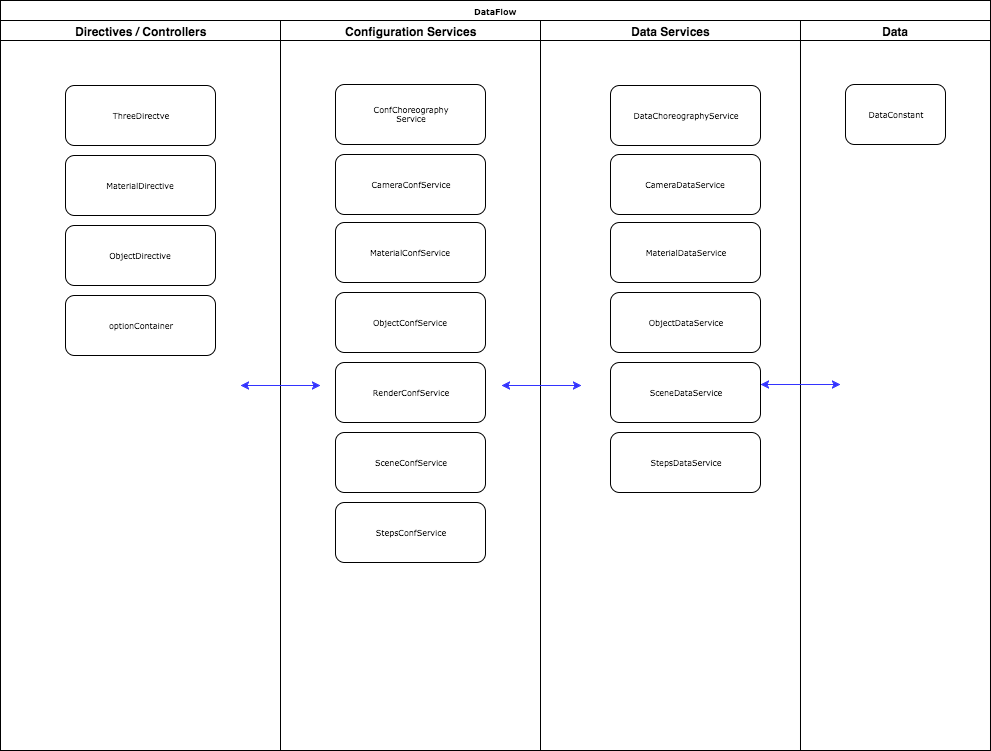
\includegraphics[width=15cm]{images/dfd}
\caption{Overview}
\label{figure:dfd}
\end{figure}
Above is a diagram with the different components. Within each column, data can flow free and can even be binded to one another. Going between columns requires a data or action call. The important thing to not here is the separation of concerns with regards to the data. The DataServices talk to the ConfigurationServices and the Data, not to the Directives / Controllers. This restricts the flow a little meaning less flexibility, but it adds clarity and makes the application less prone to bugs.


%----------------------------------------------------------------------------------------
%   Development
%----------------------------------------------------------------------------------------
\section{Development}
\subsection{Introduction}
Following below is an outline of all aims. Per aim there is a small plan of action with an expectation of the way this question may be answered.

%----------------------------------------------------------------------------------------
%   Is it possible to eliminate all issues (time and automation) with regards to rendering?
%----------------------------------------------------------------------------------------
\subsection{Is it possible to eliminate all issues (time and automation) with regards to rendering?}
This question was answered by combining the experience taken from building the prototype and the information given by Peppr. They helped outlining the current workflow so a good comparison between the current process and the hypothesized new process could be made.

%----------------------------------------------------------------------------------------
%   What is the cost differences for development?
%----------------------------------------------------------------------------------------
\subsection{What are the cost differences for development?}
To answer this question properly, a division in setup / creation costs, maintenance costs, and upgrade costs (adding components and adapting the configurator for other clients) was made. To determine the setup / creation costs, a start was made by estimating the time needed on both projects. The previously used example was used for both estimates. Combining these estimates with the hourly rates as specified by Peppr (which they claim are inline with the market) for both the development of the visuals as the development of the application makes for an estimate in cost.\newline
For the maintenance costs there were two major components that determined pricing. The first being the upgrade cycle for a CMS. The second being the upgrade cycle for a fully custom piece of software. To pin down the costs for the upgrade cycles, the average upgrade cycle was checked for both CMS and the main NPM package for the custom software (angular). Combining those with average server / deployment costs which are both needed for a CMS configurator and custom software configurator, a conclusion with regards to those costs could be made.\newline
Lastly, and this is the place were Peppr anticipated the biggest wins in terms of costs, a costs difference for adding extra options to the configurator and completely adapting it to a new situation had to be made. There was a conceptual difference in the workflows that needed to be understood as well. Eventually, the product configurators end result needs to correspond with a product number that identifies that specific configuration and / or product. This can be done quite easily by combining the numbers X-X-X (Chair Colour - Frame Number - Frame Colour). The nature of the new way of doing things means that configurations are hierarchical. A frame has to have a material and that defines the number and colour of the frame. The nature of having a property means that once adding another frame type, it can automatically inherit the property from the other frames. This means that if the chair colour and frame number and frame colour have the proper numbers, they can automatically generate a product number on the go, without specifying them.\newline
In the old situation, there was one image per configuration. This means that every time a component was added, someone had to specify the product number. As such, all the product numbers had to be entered manually (either in the file name of the image, or in the back-end) which in turn meant that every single configuration had to exist as a product in the configurator. In this case, the observed configurator was the Slimfitted configurator Peppr made earlier which used Magento as a CMS to handle the products. The software could have been written differently to handle automation of product numbers, but this could also result in overfitting.\newline
As soon as this conceptual difference was looked at, the time differences in workflows were analysed to see the differences. \newline
These three properties combined answered the question.

%----------------------------------------------------------------------------------------
%   What are the differences in Workflows
%----------------------------------------------------------------------------------------
\subsection{What are the differences in Workflows?}
Dissecting the workflow as described by Peppr and combining that with the workflow used to create the prototype gave enough information to clearly state the differences.

%----------------------------------------------------------------------------------------
%   User Experience
%----------------------------------------------------------------------------------------
\section{User Experience}
Apart from the development cycle, the user experience is a huge part of whether using these types of configurators is viable or not. Even if the development is way cheaper, if users cannot use the application, problems will arise and the old method may prove to be a better option.

%----------------------------------------------------------------------------------------
%   Is the new technology small enough?
%----------------------------------------------------------------------------------------
\subsection{Is the new technology small enough?}
This was done by recording network activity while loading the application for the SlimFitted configurator, and also for the OpenGL application. The browser used was Google Chrome, version 57.0.2987.110 with caches cleared. The following things were tested:
\label{subsub:techSmall}
​\begin{enumerate}
\item {Initial Page Load}
\item{5 colour changes (different)}
\item {2 colour changes (switch back and forth) - This is to check how Chrome caches the objects}
\item {2 component changes (different)}
\item {2 component changes (switch back and forth) - This is to check how Chrome caches the objects}
\end{enumerate}

% Record network activity for three other product configurators that have a comparable setup
% Record network activity for OpenGL version
% Find average site size
% Find psychology behind it

%----------------------------------------------------------------------------------------
%   Is the new technology small enough?
%----------------------------------------------------------------------------------------
\subsection{Is the new technology quick enough?}
To check this, loading and rendering times were recorded in as described below. Instead of running the tests with throttling for every subcomponent / colour, the throttling was only done for the initial page load. The delay in time have be extrapolated to the other components using the information from \ref{subsub:techSmall}.
​\begin{enumerate}
\item {Initial Page Load (normal)}
\item {Initial Page Load (throttled: "Regular 4G (20ms, 4.0Mb/s, 3.0Mb/s)")}
\item {Initial Page Load (throttled: "Regular 3G (100ms, 750Kb/s, 250Kb/s)")}
\item {Extrapolated page loading times with sizes specified in \ref{subsub:techSmall}}
\end{enumerate}

Another important factor for how quick the technology is, is the frames per second the graphics card can handle for the different devices. Testing this was done using a mobile low speed device (Apple iPhone 6 - 2014, retina display), a middle speed notebook (Apple Macbook - 2015, 1.1Ghz Intel Core M with Intel HD graphics, 2304 x 1440 resolution), and a high speed desktop computer (Apple Mac Pro 2013 - dual Xeon 2.7Ghz with dual AMD Firepro 500 graphics cards on two Dell 4k displays). ThreeJS statistics display was pulled from the ThreeJS example files to measure the FPS.
​\begin{enumerate}
\item {Frame 01 - Turntable}
\item {Frame 01 - Interacting}
\item {Frame 02 - Turntable}
\item {Frame 02 - Interacting}
\item {Frame 03 - Turntable}
\item {Frame 03 - Interacting}
\end{enumerate}


%----------------------------------------------------------------------------------------
%   Is the technology compatible with the users browsing preferences?
%----------------------------------------------------------------------------------------
\subsection{Is the technology compatible with the users browsing preferences?}
To test this, a browser testing tool called 'Browserstack' was used. They have something called a 'live' feature, which lets one test an application while looking at an actual device screen, unfortunately, the iPhone 7 was not supported in this manner, but as it is the latest of Apple's smartphones, it had to be included in the test. The following browsers / devices were tested:
​\begin{enumerate}
\item {Android: Samsung Galaxy S7}
\item {Android: Google Pixel}
\item {Android: LG G5}
\item {iOS: iPhone 7 --> Via iOS Simulator on 'Browserstack'}
\item {iOS: iPhone 6s}
\item {iOS: iPad Air 2}
\item {Windows 10: Edge 15}
\item {Windows 10: Firefox 53}
\item {Windows 10: Chrome 58}
\item {MacOS Sierra: Safari 10.1}
\item {MacOS Sierra: Firefox 53}
\item {MacOS Sierra: Chrome 58}
\end{enumerate}

The primary focus of the test was wether or not the application was compatible with the browsing preferences. The following things were tested for every device:
​\begin{enumerate}
\item {Did it render the chair?}
\item {Is the user able to switch colours?}
\item {Is the user able to switch frames?}
\end{enumerate}
